\chapter{Posit numbers}



\section{The posit idea}

Posit numbers made their first appearance in the work of John L. Gustfason "Beating Floating Point at its Own Game: Posit Arithmetic" \cite{gustafson2017beating}. The idea behind the format was to create a drop-in replacement for binary32 numbers. Posit numbers can be also seen as a new iteration of Universal Numbers (also called \textit{unum}). We can consider Posits as TypeIII unums.


Type I unums are a super-set of binary32 numbers, that are extended with an additional bit, called \textit{ubit}, that states whether the real number represented by that unum is an exact binary32 or lies between two consecutive representations. Another difference with binary32 numbers is that unums do not have a predefined length for exponent and fraction fields. Type I unums are also a way to represent interval arithmetic in a compact format. 

The second iteration of Type I unums - namely, Type II unums - points in the direction of totally abandoning the compatibility with binary32 numbers, nearing the concept of \textit{projective reals}.
This means that Type II unums can be projected into a ring, that wraps around from positive to negative numbers.

The final iteration of unums is represented by the Type III unum, also called Posit.


\section{Format and general properties}

Posit numbers are stored in two's complement integers. As shown in Figure \ref{fig:positFormat}, a Posit number is comprised by at most four fields. It can be configured on two parameters: the number of total bits $\text{nbits}$ and the maximum number of exponent bits $\text{esbits}$
\begin{itemize}
    \item  \textcolor{asparago}{S} is the sign bit as commonly used in IEEE binary formats.
    \item \textcolor{amber}{Regime} is the regime field, on variable length; it can take up to the entire remaining bit-space of the format.
    \item \textcolor{lightred}{Exponent} is the exponent field, without any bias offset; depending on $esbits$ and regime length it can span from $0$ to $esbits$ bits.
    \item \textcolor{lightgreen}{Fraction} is the fractional part of the mantissa; depending on the other fields it can be absent.
\end{itemize}


Sign, exponent and fraction have the same identical meaning of the homonymous fields in IEEE binary numbers. 

The regime field is instead new and different. Its length depends on the value of the bits. In particular, the regime length depends on the number of subsequent identical bits that we find after the sign, until a bit of opposite value is found. This means that, if we have this bit-string:
\begin{equation}
    b_1, b_2, b_3 \dots b_l, \overline{b_{l}}
\end{equation}
 where $b_1 = b_2 = \dots = b_l = b$, the regime length will be $l$. Depending on the value of $b$ the regime value $k$ will be computed as follows:
 
\begin{equation}\label{eqn:regimeValue}
k = \left\{\begin{matrix}
 l-1& b = 1  \\
 -l & b = 0  \\
\end{matrix}\right.
\end{equation}

The regime value is a \textit{scale factor} for a special constant, that depends on the posit configuration, called \textit{useed}. The useed value is compute as follows:
\begin{equation}\label{eqn:useed}
    \text{useed} = 2^{2^{esbits}}
\end{equation}

Wrapping everything up, the real value associated to a posit $p$ represented by the integer $P$ on two's complement (with sign $s$) is computed as in Equation \eqref{eqn:positRealValue}. The value $F$ is the length of the fraction field. Note that there will be always an implicit $1.$ in front of the fraction (i.e. $1.f_1,f_2, \dots, f_F$), without any subnormal number differently from IEEE binary numbers.

\begin{equation}\label{eqn:positRealValue}
 r =   \left\{\begin{matrix}
0 & P = 0  \\
\pm \infty & P = -2^{nbits-1}  \\
(-1)^s \cdot \text{useed}^{k} \cdot 2^e \cdot \left ( 1+ \frac{f}{2^F} \right) &  \text{otherwise} \\
\end{matrix}\right.
\end{equation}


Having the exponent and the fraction bits depending on the length of the regime is a clever way to express the so-called \textit{tapered accuracy}: numbers near $1$ (in magnitude) will have more bits allocated for the fractional part than extremely large (or small) numbers farther from $1$, thus having higher decimal accuracy. Although it highly depends on the application, the probability of encountering such extremely large or small numbers is far smaller than the one for numbers near to 1. This theoretically gives a substantial boost to posit accuracy in computations.

Figures \ref{fig:positCloseToOne} and \ref{fig:positFarFromOne} show this concept with an example. The real value $1.125$ is closer to $1$ than the value $32704$: as we can see, the number of fraction bits in the former is far greater than the one on the latter. This also reflects on the \textit{denominator} of the fraction, being $2048$ in the case of the real value $1.125$ and a quarter of that $256$ for the real value $32704$.

\begin{figure}[t]
	\centering    
    \begin{bytefield}[bitwidth=1em]{32}
       \colorbitbox{asparago}{1}{{\scriptsize{S}}}&
       \colorbitbox{amber}{10}{\scriptsize{Regime(1..$rebits$)}} &
       \colorbitbox{lightred}{9}{\scriptsize{Exponent (0..$esbits$)}} &
       \colorbitbox{lightgreen}{12}{\scriptsize{Fraction (0...)}} 
    \end{bytefield}
    \caption{The posit format}
	\label{fig:positFormat}
\end{figure}


\begin{figure}\centering\begin{bytefield}[bitwidth=0.66em]{16}\bitbox{16}{0\,1\,0\,0\,0\,0\,0\,1\,0\,0\,0\,0\,0\,0\,0\,0}\\\\\bitheader[endianness=big]{0-15}\\\colorbitbox{lightcyan}{1}{{S}}&\colorbitbox{lightgreen}{2}{R}&\colorbitbox{lightred}{2}{E}\colorbitbox{amber}{11}{F}\\\bitbox{1}{\color{cyan}0}&\bitbox{2}{\color{amber}1\!\;\color{darkamber}0}&\bitbox{2}{\color{lightred}0\!\;0}&\bitbox{11}{\color{darkgreen}0\!\;0\!\;1\!\;0\!\;0\!\;0\!\;0\!\;0\!\;0\!\;0\!\;0}&\end{bytefield}\caption{An example of Posit configuration with 16 bits and 2 exponent bits. The associated real value to the shown Posit is:$\textcolor{cyan}{1}\cdot 16^{\textcolor{darkamber}{0}}\cdot 2^{\textcolor{lightred}{0}}\cdot ( 1 + \textcolor{darkgreen}{256}/2048)= 1.125$}\label{fig:positCloseToOne}\end{figure}

\begin{figure}\centering\begin{bytefield}[bitwidth=0.66em]{16}\bitbox{16}{0\,1\,1\,1\,1\,0\,1\,0\,1\,1\,1\,1\,1\,1\,1\,1}\\\\\bitheader[endianness=big]{0-15}\\\colorbitbox{lightcyan}{1}{{S}}&\colorbitbox{lightgreen}{5}{R}&\colorbitbox{lightred}{2}{E}\colorbitbox{amber}{8}{F}\\\bitbox{1}{\color{cyan}0}&\bitbox{5}{\color{amber}1\!\;1\!\;1\!\;1\!\;\color{darkamber}0}&\bitbox{2}{\color{lightred}1\!\;0}&\bitbox{8}{\color{darkgreen}1\!\;1\!\;1\!\;1\!\;1\!\;1\!\;1\!\;1}&\end{bytefield}\caption{An example of Posit configuration with 16 bits and 2 exponent bits. The associated real value to the shown Posit is:$\textcolor{cyan}{1}\cdot 16^{\textcolor{darkamber}{3}}\cdot 2^{\textcolor{lightred}{2}}\cdot ( 1 + \textcolor{darkgreen}{255}/256)= 32704.0$}\label{fig:positFarFromOne}\end{figure}

Differently from binary32 numbers, the posit format does not have subnormal numbers. Indeed, the mantissa always has an implicit 1 and all numbers are considered in the same way. Furthermore, again in contrast with binary32 numbers, there is only one representation for infinite values or Not a Real (NaR) values. This particular bit string is represented by the integer $i = 2^{nbits - 1}$.

Given a \posit{nbits}{esbits} we can identify some important values that characterize the behaviour of the format, starting from the \textit{useed} value seen in \ref{eqn:useed}:
\[
\text{maxposit} = useed^{(nbits - 2)}
\]

\[
\text{minposit} = \frac{1}{maxposit}
\]

As explained at the beginning of this chapter, posit numbers can be projected on a circle, called \textit{posit ring}.

\begin{figure}
\centering
\begin{minipage}{.5\textwidth}
  \centering
  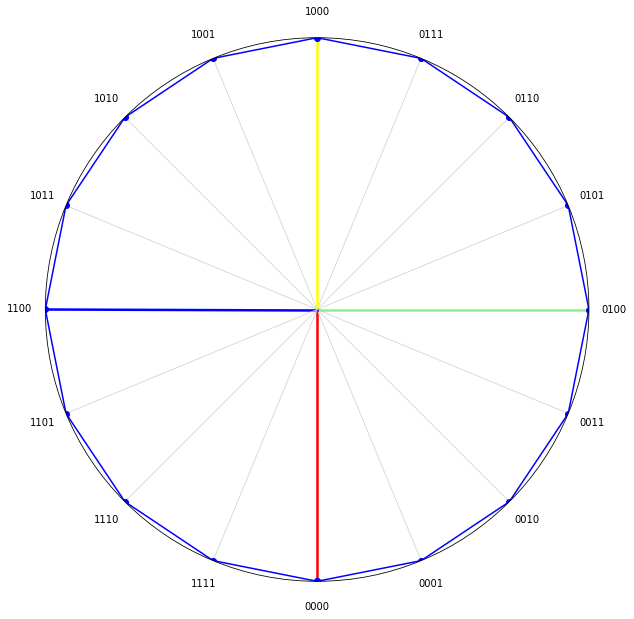
\includegraphics[width=0.9\linewidth]{img/posit4xRing.png}
  \captionof{figure}{Projection of a \posit{4}{x}}
  \label{fig:posit4xRing}
\end{minipage}%
\begin{minipage}{.5\textwidth}
  \centering
  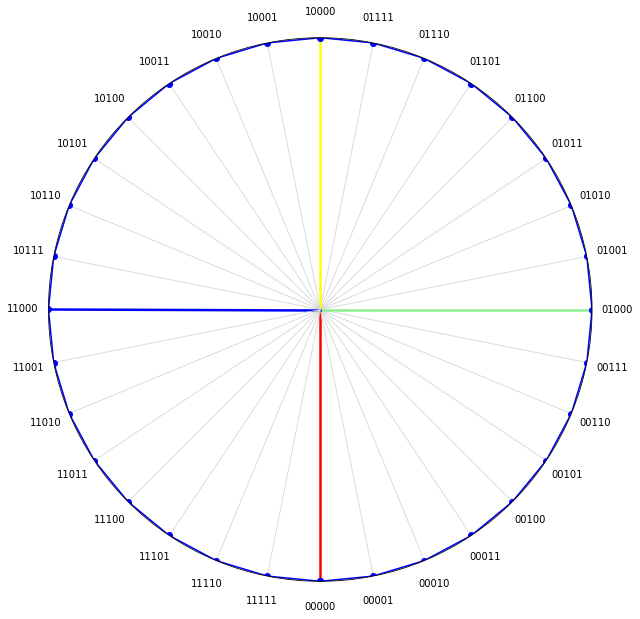
\includegraphics[width=0.9\linewidth]{img/posit5ring.png}
  \captionof{figure}{Projection of a \posit{5}{x}}
  \label{fig:posit5xRing}
\end{minipage}
\end{figure}

Figures \ref{fig:posit4xRing} and \ref{fig:posit5xRing} show the ring plot for a \posit{4}{x} and a \posit{5}{x} (exponent size is not relevant for the shape of the ring plot). The axis highlighted in \textbf{\textcolor{red}{red}} represents the real value $0$. The axis highlighted in \textbf{\textcolor{lightgreen}{green}} represents the real value $1$ and closes the first quarter of posit representations. The axis highlighted in \textbf{\textcolor{yellow}{yellow}} represents $\pm \infty$ (or \texttt{NaR}, depending on the configuration); this axis closes the quadrant where real values represented by posits are positive (note that also the integer representing the posit is positive). The axis highlighted in \textbf{\textcolor{blue}{blue}} represents the value $-1$. Note that these 4 points are fixed at south, west, north and east for any posit configuration. Indeed, they corresponds to the following posit integer representations: \textcolor{red}{0}, \textcolor{lightgreen}{$2^{nbits-2}$}, \textcolor{yellow}{$2^{nbits - 1}$} and \textcolor{blue}{$3 \cdot 2^{nbits-2}$}.

According to these two values we can explicate the rounding, overflow and underflow behaviour of the format:
\begin{itemize}
    \item If we are trying to represent a real value $0 < r < \text{minposit}$ we will saturate it to $minposit$ to avoid underflow to $0$.
    \item If we are trying to represent a real value $r > \text{maxposit} $
    \item If we are trying to represent a real value that lies between two exact posits, we need to round it to the nearest value (in terms of L2 distance).
\end{itemize}




\section{A focus on decimal accuracy}

As we said in the previous sub-section, since the posit format has a variable length field for the fraction, the decimal accuracy (i.e. the number of allocated fraction bits for a given number) varies across the posit domain.

In particular, the fraction field depends on the length of the regime and exponent fields; given a \posit{nbits}{esbits} the regime field can have a length 
\[
l_r \in [2,\text{nbits}-2]
\]
Consequently, the exponent field can have a length 
\[
l_e = \text{min}(\text{esbits},\text{nbits}-1-l_r)
\]

Finally, the fraction field can have a length:
\begin{equation}\label{eqn:fracFieldLength}
l_f = \text{nbits} - 1 - l_r - l_e
\end{equation}

Looking at the fraction field length in \ref{eqn:fracFieldLength}, we see that, when the regime value $k$ (see \ref{eqn:regimeValue}) increase in absolute value, the fraction field length decrease; this means that, when numbers are very large or very small (in absolute value) - i.e. numbers with large positive or negative regime values - the fraction field has fewer bits available for allocation. On the other hand, when the regime value decrease (in absolute value), the fraction field length increase; this means that, when numbers are very close to $1$ (in absolute value), the fraction field has more bits available for allocation. 

Having more bits available for the fraction means that we can represent more precisely numbers after the decimal dot.

\begin{figure}
    \centering
    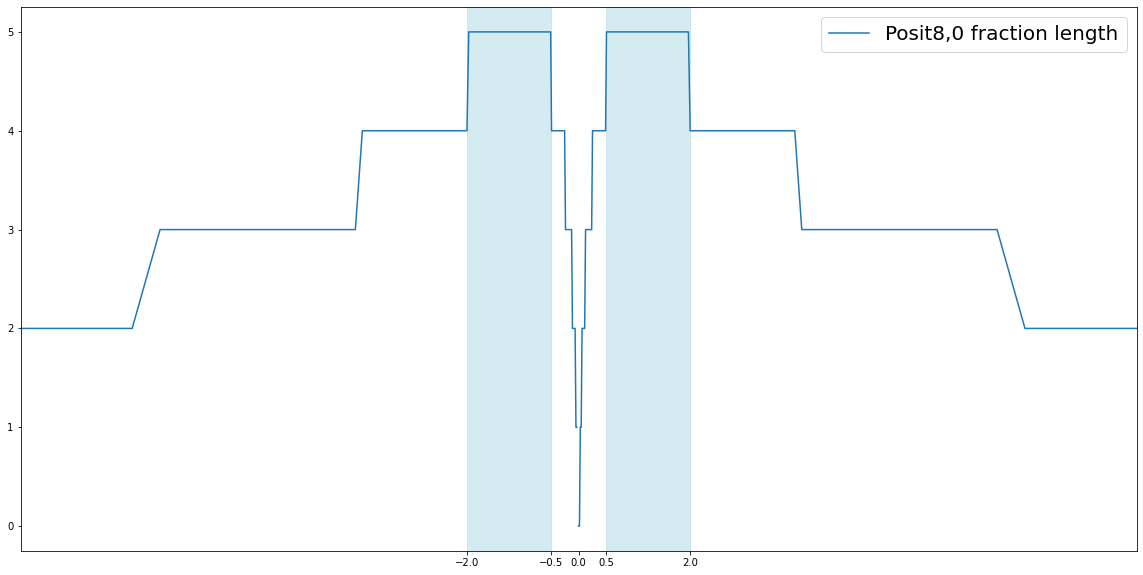
\includegraphics[width=\linewidth]{img/posit80fractionsWithZoom.png}
    \caption{\posit{8}{0} fraction length across the domain}
    \label{fig:posit80Fractions}
\end{figure}

Figure \ref{fig:posit80Fractions} shows this behaviour across the domain for a \posit{8}{0} configuration. In the plot we can see the region highlighted with the highest number of fraction bits with the associated real values $r \in [-1.9785,-0.5] \cup [0.5,1.9785]$


\begin{figure}
    \centering
    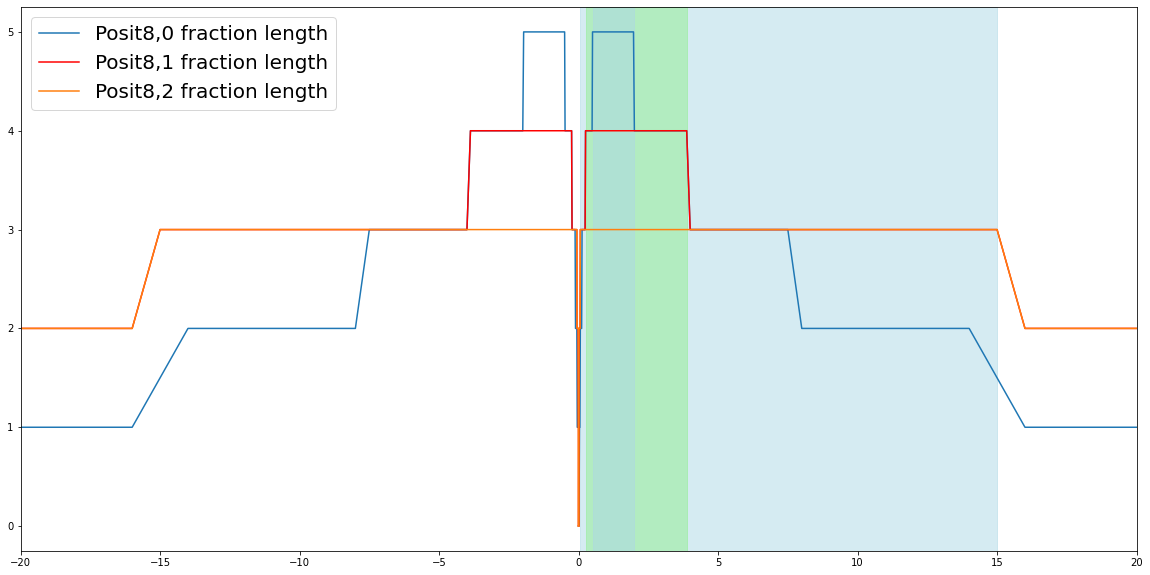
\includegraphics[width=\linewidth]{img/posit8xFractions.png}
    \caption{\posit{8}{x} fraction length comparison}
    \label{fig:posit8xFractions}
\end{figure}

Figure \ref{fig:posit8xFractions} shows the comparison of the fraction length between different configurations \posit{8}{[0,1,2]}. Obviously, if we allocate more bit for the exponent we are furtherly restricting the fraction bits, hence the different fraction bit lengths of the three configurations. However, with more exponent bits the range of maximum fraction bits is larger, despite containing the same number of distinct representations. This reflects on the format having a denser area of very high precision representation that thins out when we increase the exponent bits. 

We can generalize the range where the fraction has the highest amount of bits allocated:
\begin{equation}\label{eqn:highestFractionBits}
    \left [ \frac{1}{\text{useed}} , \text{useed} \right [ = \left [ \frac{1}{2^{2^{\text{esbits}}}}, 2^{2^{\text{esbits}}} \right [
\end{equation}

As we can see from Figure \ref{fig:posit8xFractions}, this range is always symmetric around the y-axis, so we would have the two following ranges:
\begin{equation}\label{eqn:highestFractionBitsFull}
 \left ] -\text{useed}, -\frac{1}{\text{useed}} \right ]  ; \left [ \frac{1}{\text{useed}} , \text{useed} \right [ 
\end{equation}

Note that both in \ref{eqn:highestFractionBits} and \ref{eqn:highestFractionBitsFull}, the set are open from the side of $\text{useed}$. This is because, by design, the last positive posit with the highest number fraction bits is the one immediately preceeding the posit representing $\text{useed}$.

\begin{table}[]
\caption{Ranges of the maximum fraction bits numbers for different posit configurations}
\label{tab:positXxMaxFractionRanges}
\centering
\begin{tabular}{c|rl}
Configuration               & Negative range                    & Positive range             \\ \hline
 \posit{8}{0}               & $[-1.96875, -0.5]$                  & $[0.5, 1.96875$         \\
 \posit{8}{1}               & $[-3.875, -0.25] $                  & $[0.25, 3.875]$       \\
 \posit{8}{2}               & $[-15.0, -0.0625]   $               & $[0.0625, 15.0]$         \\
 \posit{16}{0}              & $[-1.9998779296875, -0.5]$          & $[0.5, 1.9998779296875]$ \\
 \posit{16}{1}              & $[-3.99951171875, -0.25] $          & $[0.25, 3.99951171875]$  \\
 \posit{16}{2}              & $[-15.99609375, -0.0625]$           & $[0.0625, 15.99609375]$ 
\end{tabular}
\end{table}

Table \ref{tab:positXxMaxFractionRanges} summarizes the ranges of maximum fraction length for different posit configurations. As we can see the range span depends on the exponent bits (\textit{esbits}), while the decimal accuracy of the range bounds depend on the total number of bits (\textit{nbits}).

Another useful concept to understand the behaviour of posits across their domain is the \textit{resolution}. Given a pair of consecutive posit representations $p_1, p_2 = p_1 + 1; p_1, p_2 \in \mathbb{Z}$, we define resolution the value:
\begin{equation}\label{eqn:positResolution}
    \overline{r} = r_2 - r_1
\end{equation}

Where $r_1,r_2 \in \mathbb{R}$ are the real values associated, respectively, to $p_1, p_2$. Resolution represents the inverse of \textit{density} of a given format in a given range of numbers: the lower the resolution, the closer the real values associated to two consecutive representation.

\begin{figure}
    \centering
    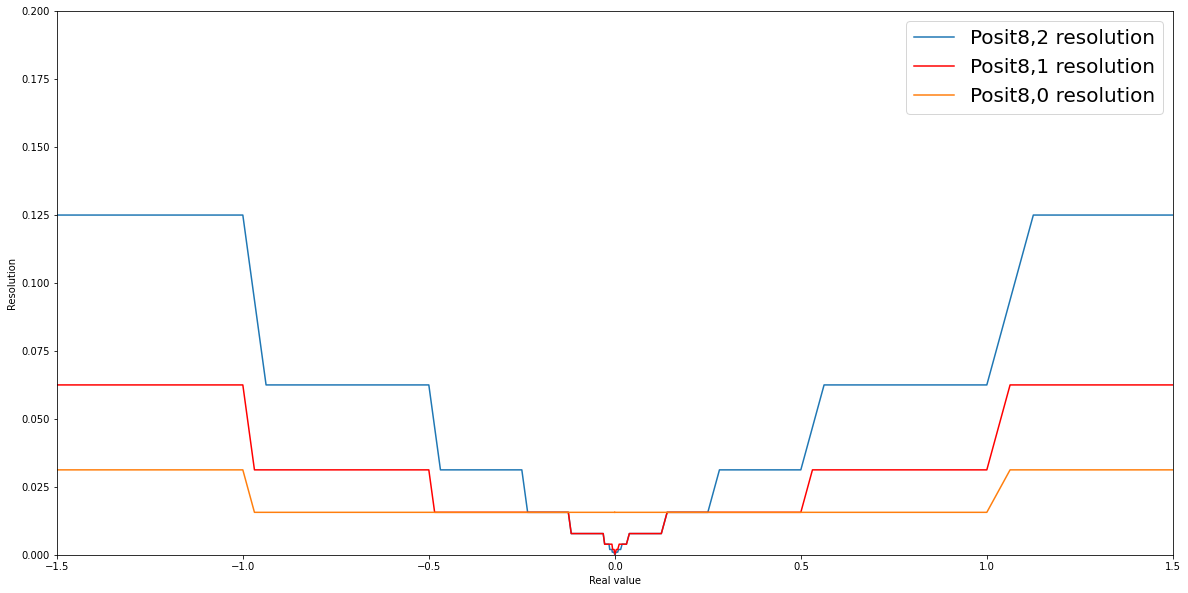
\includegraphics[width=\linewidth]{img/posit8xResolutions.png}
    \caption{\posit{8}{\{0,1,2\}} resolution across a portion of domain}
    \label{fig:posit8xResolutions}
\end{figure}

Figure \ref{fig:posit8xResolutions} shows the plot of $\overline{r}$ when function of $p_1$ for three configurations of \posit{8}{x}. As we can see, the \textit{resolution} decreases when approaching the value $0$ on the x-axis. Furthermore, the value of $\overline{r}$ is always smaller when using less exponent bits, this means that, real numbers represented by successive posits are closer if compared to other posit configurations with higher number of bits. As reported, the configurations for \posit{x}{0} have a flat resolution in the range $\left [ -1, 1 \right]$. This behaviour will be deeply analyzed in Section \ref{sec:Posit0bitExponent}.

\section{Posit $\Leftrightarrow$ Floating point  interoperability}

One of the core concepts we deal with when bringing together the posit and the floating point domains is the interoperability between the two worlds. This means that we need to have a couple of functions $f,g$ such that, given a set of Posits $\mathbb{P}$ and a set of floating point $\mathbb{F}$:
\begin{equation}
    f: \mathbb{P} \xrightarrow[]{} \mathbb{F}
\end{equation}
\begin{equation}
    g: \mathbb{F} \xrightarrow[]{} \mathbb{P}
\end{equation}

Note that these two functions must be independent from the posit configuration \posit{nbits}{esbits} and the floating point type.

We introduce a \textit{float intermediate representation} (FIR) - i.e. a contact interface between any posit and any float configuration. Similarly to an IEEE binary, a FIR interface has three fixed-length fields:
\begin{itemize}
    \item sign $s_f$ on $1$ bit
    \item exponent $e_f$ on $\text{E}_f$ bits
    \item fraction $f_f$ on $\text{F}_f$ bits
\end{itemize}

Differently from the IEEE binary formats, the exponent here is a \textit{pure} one, without any offset applied. This means that, the correspondent real value $r$ is:
\begin{equation}\label{eqn:firEquation}
    r = (-1)^{s_f} \cdot 2^{e_f} \cdot \left(1 + \frac{f_f}{2^{F_f}} \right)
\end{equation}

This interface allows us to decouple any posit configuration from any floating point configuration for conversion. Instead, we define another couple of functions $f_{fir}, 
g_{fir}$ that convert a posit into the FIR space and vice-versa.

From the other side, we just need to provide yet another couple of functions for conversion between FIR and floating point space.

We can now characterize the two functions $f_{fir}, g_{fir}$ comparing Equations \eqref{eqn:positRealValue} and \eqref{eqn:firEquation}. If we take the general case from \eqref{eqn:positRealValue} and we expand the $useed$ term with \eqref{eqn:useed} we obtain:
\begin{equation}\label{eqn:positRealExpanded}
    r = (-1)^s_p \cdot 2^{2^{esbits} \cdot k + e_p} \cdot \left ( 1+ \frac{f_p}{2^{F_p}} \right)
\end{equation}

If we compare Equation \eqref{eqn:positRealExpanded} and \eqref{eqn:firEquation} we can impose equality on the three terms of the multiplication. The sign equality is straightforward: the sign of the number in FIR format will match the posit one.

If we are converting from posit to FIR, we can obtain the exponent $e_f$ as:
\begin{equation}
    e_f = 2^{esbits} \cdot k + e_p
\end{equation}

If we are converting the other way we can obtain $k$ and $e_p$ using modular arithmetic in base $2$.
\begin{equation}
    k = e_f\ \mathbf{mod}\ 2^{esbits} = \left\lfloor \frac{e_f}{2^{esbits}} \right\rfloor
\end{equation}

\begin{equation}
    e_p = e_f\ \mathbf{rem}\ 2^{esbits}
\end{equation}

Where $\mathbf{mod}$ is the integer division quotient and $\mathbf{rem}$ is the remainder.

For the fraction we need to impose the equality:
\begin{equation}\label{eqn:fractionalPartEquivalence}
    \frac{f_f}{2^{F_f}} = \frac{f_p}{2^{F_p}}
\end{equation}

Then we can solve for $f_f$ as:
\begin{equation}
    f_f = f_p \cdot 2^{F_f - F_p}
\end{equation}

and we can solve for $f_p$ as:
\begin{equation}
    f_p = f_f \cdot 2^{F_p - F_f}
\end{equation}

Note that, depending on the fraction sizes, the operation may result in loss of information, when we shrink a fraction with more bits to one with less bits.  Therefore, we need to take into account the bits we are discarding to eventually round the destination format according to their value.

So far, we have covered the conversion between FIR and posit numbers. The conversion between FIR and actual IEEE binary (or whichever floating point format) is similar, if not simpler.

Let us consider the IEEE binary32 conversion from/to a given FIR format. 

The exponent $e_{b32}$ of a binary32 number must be offset by $127$ during transition between the two formats. Therefore, given $e_f$ the FIR exponent, we obtain:
\begin{equation}
    e_{b32} = e_f + 127
\end{equation}

On the other hand:
\begin{equation}
    e_{f} = e_{b32} - 127
\end{equation}

The fractional part can be handled as in \ref{eqn:fractionalPartEquivalence}. Note that, differently from posit numbers, when the exponent is $0$, the fractional part of a binary32 needs to be interpreted without the leading $1.$ (i.e. the number must be considered as a subnormal).

The approach of using an intermediate representation can be used between whichever formats for real numbers that can be represented in the sign, exponent and fraction format.

\cfr{Qualche esempino, anche con un subnormal}

\section{Generalized posits}

As seen in Figures \ref{fig:posit80Fractions} and \ref{fig:posit8xFractions}, the regime length has a sensible impact on the number of fraction bits we can use across the domain. Such length can change to the point where we do not have sufficient decimal accuracy in a given range of numbers. 

An ideal approach would be to impose an upper limit to the regime length such that we can be sure that we will always reserve at least some bits for the fraction.

In \cite{9151086}, the authors propose a new way to characterize a posit numbers. Additionally to the \textit{nbits}  and \textit{esbits} parameters, there are two (mutually exclusive) new hyper-parameters that control the dynamic range:
\begin{itemize}
    \item $K_b$: a regime bias 
    \item $rs$: a limit on the regime length
\end{itemize}

This results in having the maximum posit value shifted at:
\begin{equation}
    2^{2^{esbits} \cdot (k-K_b)}
\end{equation}

if using the $K_b$ parameter, or if we use the $rs$ parameter:
\begin{equation}
    2^{2^{esbits} \cdot rs} \cdot (1 - 2^{es - t - 1})
\end{equation}

where $ t = n - rs - 1$
\section{A special case: 0-bit exponent}\label{sec:Posit0bitExponent}

In this Section we focus on the posit format when configured with 0 exponent bits (i.e. \posit{x}{0}). If we impose $esbits = 0$ - that means also $es = 0$ - in \ref{eqn:positRealValue}, we get:
\begin{equation}\label{eqn:positRealValueExp0}
    (-1)^s \cdot \text{2}^{k} \cdot \left ( 1+ \frac{f}{2^F} \right)
\end{equation}

since $useed = 2^{2^0} = 2$. T


